% Midpoint report, CS 59300-ASE. Rebuilt from Vedant's draft (abstract, introduction, Section 2)
% with the updates in abstract_intro_edits.tex applied, plus Sections 3 and 4.
% Build: tectonic main.tex
\documentclass[sigconf,review]{acmart}

\usepackage{tikz}
\usetikzlibrary{positioning}

\settopmatter{printacmref=false}
\setcopyright{none}
\renewcommand\footnotetextcopyrightpermission[1]{}
\acmConference[CS 59300-ASE]{CS 59300-ASE}{Fall 2026}{West Lafayette, IN}
\acmYear{2026}
\acmDOI{}
\acmISBN{}

% Student IDs live in ids.tex, which is not committed (the repository is public). Without it the
% PDF shows names only. ids.tex holds: \renewcommand{\vedantid}{ (0...)} \renewcommand{\yashid}{ (0...)}
\newcommand{\vedantid}{}
\newcommand{\yashid}{}
\InputIfFileExists{ids.tex}{}{}

\begin{document}

\title[Reliability Regressions in AI-Maintained Microservices]{It Worked Yesterday: Detecting and Repairing Reliability Regressions in Microservices Maintained by AI Coding Agents}

\author{Vedant Prabhu\vedantid}
\affiliation{%
  \institution{Purdue University}
  \city{West Lafayette}
  \state{Indiana}
  \country{USA}}
\email{prabhu76@purdue.edu}

\author{Yash Tembhurnikar\yashid}
\affiliation{%
  \institution{Purdue University}
  \city{West Lafayette}
  \state{Indiana}
  \country{USA}}
\email{ytembhur@purdue.edu}

\renewcommand{\shortauthors}{Prabhu and Tembhurnikar}

\begin{abstract}
AI coding agents are no longer used only to write new code. Teams
now ask them to keep changing existing systems: add a service, add
a cache, change how retries work. Each of these changes is usually
checked with functional tests, which tell us whether the new feature
works. They do not tell us whether the change quietly broke how
the system behaves when something goes wrong, such as a slow
dependency, a crashed service, or a lost response. In a microservice
application these failures are normal, and code that handles them
badly causes hung requests, retry storms, and duplicate payments.
We call this kind of silent breakage a \emph{reliability regression}.

We propose a project with two parts. First, an empirical study
of how often reliability regressions appear when AI coding agents
make a sequence of changes to the same microservice application,
which kinds of changes cause them, and which kinds of faults
expose them. Second, a tool, \textsc{ReliGuard}, that runs after every
AI-made change. It injects realistic faults, re-checks every reliability
property the system satisfied before the change, and when one fails,
gives the agent structured evidence about the failure and verifies
the agent's fix against the full set of properties. We have built a
checkout application of three services and a database with network
fault injection, and written ten reliability properties as executable
checks before any agent touched it. The checks pass on every run
of the baseline and catch five of six faults we planted on purpose;
our functional tests catch only one.
We will drive three coding agents (Claude Code, Codex CLI, and
GitHub Copilot's coding agent) through the same sequence of eight
changes, three times each, measure regression rates per change and
per fault type, and compare \textsc{ReliGuard}'s repair feedback against
a plain ``here is the error, fix it'' baseline. In a pilot, Claude Code
completed the first two changes with all of its own tests passing,
yet its second change broke three of the ten properties: checkout
under a slow payment service now took 18\,s to answer instead of under
3\,s, and a failing payment was attempted 11 times instead of at most 3.
\end{abstract}

\begin{CCSXML}
<ccs2012>
<concept><concept_id>10011007.10011074.10011099.10011102.10011103</concept_id>
<concept_desc>Software and its engineering~Software testing and debugging</concept_desc>
<concept_significance>500</concept_significance></concept>
<concept><concept_id>10011007.10011074.10011111.10011113</concept_id>
<concept_desc>Software and its engineering~Software evolution</concept_desc>
<concept_significance>300</concept_significance></concept>
<concept><concept_id>10010520.10010575</concept_id>
<concept_desc>Computer systems organization~Dependable and fault-tolerant systems and networks</concept_desc>
<concept_significance>300</concept_significance></concept>
</ccs2012>
\end{CCSXML}
\ccsdesc[500]{Software and its engineering~Software testing and debugging}
\ccsdesc[300]{Software and its engineering~Software evolution}
\ccsdesc[300]{Computer systems organization~Dependable and fault-tolerant systems and networks}

\keywords{AI coding agents, reliability regression, microservices, fault injection, automated program repair}

\maketitle

\section{Introduction}

\textbf{Background.} AI coding agents such as Claude Code, Codex CLI,
and GitHub Copilot's coding agent can now read a repository, edit
many files, run commands, and open a pull request with little human
help. Most of the evidence that they work comes from benchmarks
like SWE-bench~\cite{jimenez2024swebench}, where an agent fixes one issue in one snapshot
of a repository and is graded by the project's tests. Real software
does not stop after one change, though. It keeps evolving, and
more and more of that evolution is being handed to agents. There
are early signs that this has a cost. The 2024 DORA report found
that as teams adopted more AI assistance, their software delivery
stability went \emph{down}, by an estimated 7.2\% for every 25\% increase in
AI adoption~\cite{dora2024}. Faster code changes are not the same as safer ones.

\textbf{The problem.} We are interested in one specific way this goes
wrong. Consider a small online store built from an Order service that
calls a Payment service and an Inventory service. The Order service
already handles a slow Payment service correctly: it gives up after
a second and returns a clear error. Now we ask an agent to ``add
a Notification service that emails the user after checkout.'' The agent
does it, and the new notification test passes. But while wiring in the
new call, it also replaced the HTTP client in the Order service and
dropped the timeout. Nothing in the functional tests notices. The
next time Payment is slow, every checkout request hangs, threads
pile up, and the whole store stops responding. The new feature
works; an old guarantee is gone. We call this a \emph{reliability regression}:
a property about behavior under failure (bounded latency, safe
retries, no duplicate side effects, recovery after an outage) that held
before a change and no longer holds after it. These regressions
are easy to introduce in microservices because a small edit in one
service changes how it behaves toward every service it calls, and
they are hard to see because they only appear when something
fails. Retry logic alone is a well known source of production bugs
even in mature, human-written systems~\cite{stoica2024retry}. If agents are going to
maintain these systems, we need to know whether they preserve
these guarantees over time, and we need a way to catch and repair
the cases where they do not.

The goal of this project is to (1) measure how often, where,
and why reliability regressions appear when AI agents repeatedly
modify a microservice system, and (2) build and evaluate a tool
that detects these regressions after each change and helps the agent
repair them without breaking something else.

\textbf{Existing work and its limits.} Four lines of work come close,
but none answers our question. \emph{Agent evaluation over time.} Evo\-Claw~\cite{deng2026evoclaw}
and SWE-EVO~\cite{le2025sweevo} evaluate agents on long sequences
of changes to the same codebase, which is the setting we care
about. However, they judge each step only with functional tests,
so a change that breaks failure handling but keeps the tests green
counts as a success. \emph{Reliability of AI-written code.} Tao et al.~\cite{tao2026observability}
injected faults into microservice code written by coding agents and
found that the code exposed useful fault signals for at most about
14\% of failures. Earlier work showed that Copilot code that looks
correct is often insecure~\cite{pearce2022asleep}. Both studies look at code produced
in one shot, not at what happens to a system as an agent keeps
changing it. \emph{LLMs for operations.} MicroRemed~\cite{zhang2025microremed} benchmarks
LLMs that repair injected microservice failures by writing Ansible
playbooks, and ChaosEater~\cite{kikuta2025chaoseater} uses LLM agents to plan and run
chaos engineering experiments. In both, the LLM operates or tests
a system that humans wrote; it is not the developer whose own
changes caused the failure. \emph{Resilience testing.} Chaos engineering~\cite{basiri2016chaos}
and fault-injection tools such as Gremlin~\cite{heorhiadi2016gremlin} and Filibuster~\cite{meiklejohn2021filibuster}
give us the techniques to expose failure-handling bugs, but they
were designed for human-written code and do not connect their
findings back to an agent that can fix them. To our knowledge, no
prior work tracks whether reliability properties survive a \emph{sequence}
of AI-made changes, or closes the loop by feeding fault-injection
evidence back to the agent that caused the regression.

\begin{figure}[t]
  \centering
  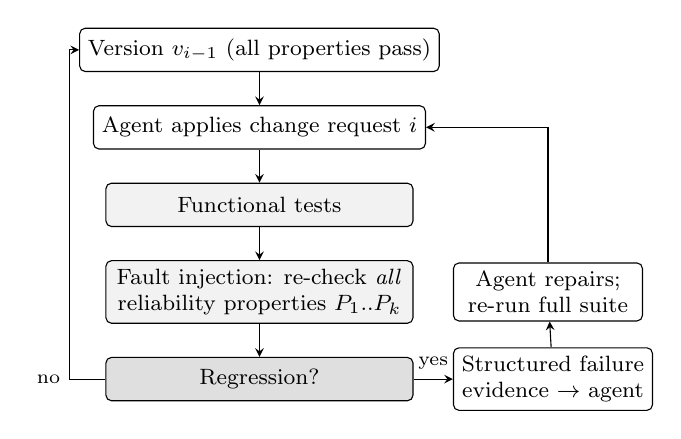
\begin{tikzpicture}[font=\footnotesize, >=stealth, node distance=0.42cm,
      flow/.style={draw, rounded corners=2pt, align=center, inner sep=3pt, minimum height=0.55cm, minimum width=3.9cm},
      side/.style={draw, rounded corners=2pt, align=center, inner sep=3pt, minimum height=0.55cm, minimum width=2.4cm}]
    \node[flow] (v) {Version $v_{i-1}$ (all properties pass)};
    \node[flow, below=of v] (apply) {Agent applies change request $i$};
    \node[flow, fill=gray!10, below=of apply] (func) {Functional tests};
    \node[flow, fill=gray!10, below=of func] (fault) {Fault injection: re-check \emph{all}\\reliability properties $P_1..P_k$};
    \node[flow, fill=gray!25, below=of fault] (reg) {Regression?};
    \node[side, right=0.5cm of reg] (evid) {Structured failure\\evidence $\rightarrow$ agent};
    \node[side, right=0.5cm of fault] (repair) {Agent repairs;\\re-run full suite};
    \draw[->] (v) -- (apply);
    \draw[->] (apply) -- (func);
    \draw[->] (func) -- (fault);
    \draw[->] (fault) -- (reg);
    \draw[->] (reg) -- node[above, font=\scriptsize] {yes} (evid);
    \draw[->] (evid) -- (repair);
    \draw[->] (repair.north) |- (apply.east);
    \draw[->] (reg.west) -- ++(-0.45,0) node[pos=1, left, font=\scriptsize] {no} |- (v.west);
  \end{tikzpicture}
  \caption{\textsc{ReliGuard}'s loop, run after every agent change. The study records what happens
  at each step; the tool automates detection, feedback, and repair verification.}
  \label{fig:loop}
\end{figure}

\textbf{Our approach.} Our project combines a study with a tool, and
the tool is the infrastructure that makes the study possible. We
describe it using the design argument framework: a goal, the design
choices we make, and why each choice serves the goal. The \emph{goal}
of \textsc{ReliGuard} is to make sure that an agent's change does not
silently weaken how the system behaves under failure, and that
any weakening it does introduce gets fixed. Figure~\ref{fig:loop} shows the
loop. It rests on four design choices. \emph{(D1) Reliability properties are
written as executable checks before any agent touches the code.} Each
check pairs a fault with an expected behavior, for example ``when
Payment adds 5\,s of latency, a checkout returns an error within
3\,s'' or ``when Payment's response is dropped after it charged the
card, the retried checkout does not charge twice.'' Writing them
up front gives us an objective, repeatable definition of a regression
instead of a judgment call after the fact. \emph{(D2) Every check runs after
every change, not only the checks related to the change.} Regressions,
by definition, show up in behavior the change was not supposed
to touch, so only a full re-run catches them. \emph{(D3) When a check
fails, the agent gets structured evidence rather than a raw log dump:}
which fault was injected, which property was expected, what was
observed (for example, ``46 retries, request never returned''), the
relevant request trace, and the diff that introduced the problem. Our
hypothesis is that agents repair failures better when they can see
the cause and the scope, instead of guessing from symptoms. \emph{(D4) A
repair is only accepted if the entire property suite passes again.} Agents
sometimes ``fix'' one failure by breaking another, so the original
failing check alone is not enough.

\textbf{Study plan.} \emph{Subject system.} We built a four-service checkout
application (Order, Payment, Inventory, and a database), loosely
modeled on the checkout path of Google's Online Boutique~\cite{onlineboutique}. It runs
locally with docker-compose, so the whole experiment costs nothing,
and will move to Kubernetes (Kind) with Chaos Mesh~\cite{chaosmesh} for pod-level
faults after the midpoint. Faults are injected with Toxiproxy~\cite{toxiproxy}: added
latency, an unavailable service, bursts of HTTP 503 errors, responses
lost after the server has acted, and duplicate request delivery.
Version~0 passes all functional tests and all ten reliability properties
(12 checks covering bounded latency, bounded retries, graceful
errors, idempotency, recovery after an outage, and Order/Inventory
consistency). \emph{Change sequence.}
Each agent receives the same eight change requests in the same
order: add a Notification service, add retries to payment calls, add
caching, add rate limiting, move notifications to a message queue,
change a database interaction, add a new API endpoint, and adjust
timeout settings. Each change starts from the agent's own previous
version, so mistakes can accumulate, as they would in a real codebase. \emph{Agents and runs.}
We will use three agentic tools that edit the
repository directly (Claude Code, Codex CLI, and GitHub Copilot's
coding agent) with pinned model versions, identical prompts, and
no human edits to the code. Because agents are nondeterministic,
each agent runs the full sequence three times, giving 3 agents $\times$ 3
runs $\times$ 8 changes = 72 evolved versions. We will answer three research questions.
\textbf{RQ1:} How often do reliability regressions appear
as agents make sequential changes, and do they accumulate over
the sequence? We measure the fraction of versions with at least one
regression, the number of properties broken per version, and how
this changes from change 1 to change 8, alongside the functional
pass rate for contrast. \textbf{RQ2:} Which kinds of changes introduce
regressions, and which kinds of faults expose them? We tabulate
regressions by change type and fault type, and manually categorize
the root causes (for example, removed timeout, unbounded retry,
missing idempotency key). \textbf{RQ3:} Can agents repair the regressions,
and does \textsc{ReliGuard}'s structured feedback help? For each regression we compare two feedback conditions given to the same agent:
\textsc{ReliGuard}'s structured evidence versus a baseline that only passes
the failing test's name and raw log. We measure repair success
(original check passes), clean repair rate (the whole suite passes),
and collateral regressions introduced by the repair.

\textbf{Feasibility and division of work.} Both authors have production
backend experience. Yash will lead the services, Kubernetes
setup, and fault injection; Vedant will lead the property checks, the
agent harness that applies change requests and collects results, and
the repair experiment. At the midpoint, Version~0 and all property checks are complete
and validated, and a pilot run of Claude Code through the first two
changes is done; the full runs follow (Section~\ref{sec:method}). Two threats we are aware of: because we build
Version~0 ourselves, it may not represent real systems, so we will
keep it close to Online Boutique's design and release all prompts
and code; and a single subject application limits generality, which
we will state clearly and treat as the main direction for future work.

\textbf{Expected contributions.} (1) The first study, to our knowledge,
of reliability regressions across sequences of AI-made changes; (2)
\textsc{ReliGuard}, an open-source tool that detects these regressions and
feeds structured evidence back to the agent; and (3) a reusable
benchmark of a microservice application, change sequence, and
reliability properties that others can use to evaluate future coding
agents on more than ``do the tests pass.''

The rest of this report is organized as follows. Section~\ref{sec:related} reviews related work,
Section~\ref{sec:method} describes our method and the progress so far, and
Section~\ref{sec:expected} gives our expected findings and evaluation plan.

\section{Related Work}
\label{sec:related}

Our project sits where four lines of work meet: evaluating AI coding agents, studying the quality
of code those agents write, using LLMs to operate and test cloud systems, and resilience testing of
microservices. We go through each in turn and end with what is still missing.

\subsection{Evaluating coding agents, from one change to many}

Most of what we know about coding agents comes from SWE-bench~\cite{jimenez2024swebench}. Each task
is one GitHub issue in one snapshot of a Python repository, and the agent's patch counts as correct
if the project's own tests pass afterwards. Agent designs such as SWE-agent~\cite{yang2024sweagent}
and simpler pipelines such as Agentless~\cite{xia2025agentless} were both developed and compared on
this setup. SWE-bench made agent evaluation concrete and repeatable, but every task starts from a
clean snapshot and ends after one patch, so it cannot show what happens when an agent keeps working
on code it changed itself.

Two recent benchmarks move toward that setting. SWE-EVO~\cite{le2025sweevo} gives agents
long-horizon evolution tasks that require many coordinated changes, and EvoClaw~\cite{deng2026evoclaw}
goes further by replaying a repository's real development history as a sequence of milestones, so
later tasks build on the agent's own earlier output. This is the closest setting to ours. The
difference is the oracle. Both benchmarks judge each step with functional tests: if the tests pass,
the step succeeds. A change that removes a timeout or makes a retry loop unbounded usually keeps
every functional test green, because the tests never make a dependency slow or unavailable. Our
study keeps the sequential setting but changes what is checked after every step.

\subsection{Quality of AI-written code beyond correctness}

A second line of work asks whether code that passes its tests is actually good. Pearce et
al.~\cite{pearce2022asleep} generated programs with GitHub Copilot for scenarios tied to known
weakness types and found that about 40\% of them were vulnerable, even though they looked
reasonable. Closer to our topic, Tao et al.~\cite{tao2026observability} asked coding agents to build
or restore observability in microservice applications, injected faults, and found that the
resulting systems exposed a useful fault signal for at most about 14\% of failures, despite
producing plenty of log lines. Both studies show that functional correctness says little about how
AI-written code behaves in the cases that matter in production.

What these studies share is that the code is produced once and then measured. They do not tell us
whether properties that already hold in a system survive when an agent edits it, which is the
situation most teams are in. In our setting Version~0 is known to satisfy every reliability
property, so any failure afterwards can be traced to a specific agent change.

\subsection{LLMs for operating and testing cloud systems}

LLMs are also being used on the operations side. MicroRemed~\cite{zhang2025microremed} injects
failures into microservice systems, gives an LLM a diagnosis, and checks whether the Ansible
playbook it writes actually repairs the system. ChaosEater~\cite{kikuta2025chaoseater} automates
the whole chaos engineering cycle with LLM agents: it writes hypotheses, plans fault-injection
experiments on Kubernetes, runs them, and proposes changes to the system configuration. These works
show that LLMs can reason about faults in distributed systems and act on the results of fault
injection.

In both cases, however, the LLM is working on a system someone else wrote. The failures it handles
are injected into the infrastructure, not introduced by the LLM's own code changes. Our project
looks at the opposite direction: the agent is the developer, the regression is caused by its
change, and fault injection is the way we find out.

\subsection{Resilience testing of microservices}

Testing how a distributed system behaves under failure is an established practice. Netflix's chaos
engineering~\cite{basiri2016chaos} runs controlled experiments that inject failures into production
to check that the system still meets its steady-state behavior. Gremlin~\cite{heorhiadi2016gremlin}
brought this into testing by injecting faults at the network layer between microservices and
checking assertions about how services respond, and Filibuster~\cite{meiklejohn2021filibuster}
systematically injects service-level faults during functional tests to find failure-handling bugs.
Stoica et al.~\cite{stoica2024retry} studied retry bugs in mature open-source systems and found that
retry logic, which looks simple, is a common source of real failures: missing retries, unbounded
retries, and retries that repeat side effects. These tools and findings are the reason we chose
bounded latency, bounded retries, idempotency, and recovery as our properties, and
Toxiproxy~\cite{toxiproxy} is how we inject the faults.

Resilience testing was designed for human-written code, and its output is a report for a human
engineer. It also has no notion of a sequence of versions. The classic answer to ``did this change
break something that used to work'' is regression testing~\cite{yoo2012regression}, but regression
suites are almost always functional. Our property suite is in effect a regression suite for failure
behavior, re-run in full after every agent change.

\subsection{Feeding failures back to the model}

\textsc{ReliGuard}'s repair step builds on work showing that LLMs fix code better when they get
execution feedback. Self-Debugging~\cite{chen2024selfdebug} has the model run its code and explain
the result to itself before revising, and ChatRepair~\cite{xia2024chatrepair} repairs bugs through
a conversation that feeds failing test output back to the model after each attempt. Both use
functional test failures as the feedback. We give the agent a different kind of evidence: which
fault was injected, which property was expected, what was observed, and which diff introduced the
regression. We also accept a repair only if the whole property suite passes, because a fix that
restores one property by breaking another is not a fix.

\subsection{The gap}

Putting these together: agent benchmarks follow systems over many changes but only check functional
behavior; studies of AI-written code check non-functional behavior but only for code written once;
LLM operations work uses fault injection but on systems the LLM did not write; and resilience
testing has the techniques but no connection to an agent that could fix what it finds. To our
knowledge no prior work measures whether reliability properties survive a sequence of AI-made
changes, or closes the loop by giving fault-injection evidence back to the agent that caused the
regression. That is the gap this project addresses.

% ---------------------------------------------------------------------------------------------
% Section 3: Method and Progress (#15). Paste after Section 2 (Related Work), before References.
% Needs \usepackage{tikz} (already used by Figure 1) and booktabs (loaded by acmart).
% Citation keys: rename to match the project's .bib if they differ (see README.md in this folder).
% ---------------------------------------------------------------------------------------------

\section{Method and Progress}
\label{sec:method}

Our project is an empirical study whose instrument is a tool. This section describes the
components we have built, how we check that they measure what we claim, what the first agent
runs show, and what remains. Everything described here is in a public repository with
continuous integration,\footnote{\url{https://github.com/Yash-11-star/religuard}. Version~0 is tag
\texttt{v0}; the results below are under \texttt{results/} (\texttt{v0/}, \texttt{mutants/},
\texttt{pilot/}).} and every number below can be reproduced with the scripts in it.

\subsection{Changes since the proposal}
\label{sec:scope}

We made one scope change. The proposal ran the subject system on Kubernetes (Kind) with
Chaos Mesh~\cite{chaosmesh}. For the midpoint we built it on docker-compose instead and inject
all faults with Toxiproxy~\cite{toxiproxy}. Every fault our properties need (added latency,
an unreachable service, responses lost after the server acted) is a network fault that Toxiproxy
produces directly, and docker-compose let us reach a stable baseline and a first agent run in
the time available. Moving to Kind and adding Chaos Mesh for pod-level faults (container kills,
restarts) is the first milestone after the midpoint (Section~\ref{sec:remaining}). The research
questions, the three agents, the eight changes, and the 72-version design are unchanged.

\subsection{Subject system: Version 0}
\label{sec:v0}

Version~0 is a checkout service built from three Python (FastAPI) services and a PostgreSQL
database (Figure~\ref{fig:arch}). \emph{Order} receives \texttt{POST /checkout}, reserves stock in
\emph{Inventory}, charges the customer through \emph{Payment}, and then commits or releases the
reservation. Every call from Order to its dependencies, including to its own database, passes
through Toxiproxy, so a test can slow down, cut off, or silence any dependency without changing
any code. Payment and Inventory also expose small \texttt{/admin} endpoints that let a check count
charges and attempts, read stock levels, and force HTTP 503s or card declines, which Toxiproxy
cannot produce.

We wrote Version~0 to be correct under failure, using the patterns that the retry-bug study of
Stoica et al.~\cite{stoica2024retry} identifies as commonly gotten wrong:
(i)~a 1\,s timeout on every attempt and a 2.5\,s deadline for the whole checkout, so a slow
dependency cannot make checkout hang;
(ii)~at most three attempts with jittered exponential backoff, retrying only timeouts, connection
errors, and 502/503/504;
(iii)~the same idempotency key (\texttt{order-<id>}) on every charge attempt, and an idempotency key
on the checkout request itself, so neither retries nor duplicate deliveries charge twice;
(iv)~compensation: a failed or abandoned checkout releases its stock reservation, and a background
task finishes or fails every order, so none stays \texttt{PENDING}; and
(v)~a 1\,s bound on each database statement.
These mechanisms are exactly what an agent can quietly remove while adding a feature.

\begin{figure}[t]
  \centering
  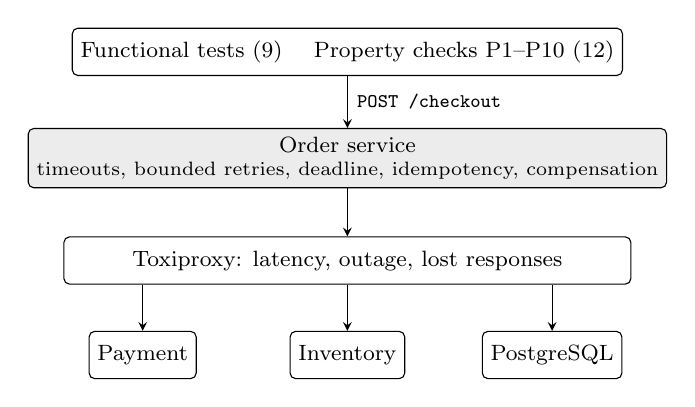
\begin{tikzpicture}[font=\footnotesize, >=stealth,
      box/.style={draw, rounded corners=2pt, align=center, inner sep=3pt, minimum height=0.6cm}]
    \node[box] (checks) at (0,2.5) {Functional tests (9) \quad Property checks P1--P10 (12)};
    \node[box, fill=gray!15] (order) at (0,1.15) {Order service\\[-1pt]
      \scriptsize timeouts, bounded retries, deadline, idempotency, compensation};
    \node[box, minimum width=7.2cm] (tox) at (0,-0.15) {Toxiproxy: latency, outage, lost responses};
    \node[box] (pay) at (-2.6,-1.35) {Payment};
    \node[box] (inv) at (0,-1.35) {Inventory};
    \node[box] (db) at (2.6,-1.35) {PostgreSQL};
    \draw[->] (checks) -- node[right, font=\scriptsize] {\texttt{POST /checkout}} (order);
    \draw[->] (order) -- (tox);
    \draw[->] (tox.south -| pay) -- (pay);
    \draw[->] (tox) -- (inv);
    \draw[->] (tox.south -| db) -- (db);
  \end{tikzpicture}
  \caption{Version~0. The checks drive checkout over HTTP, inject faults through Toxiproxy's API,
  and read the outcome from the services' \texttt{/admin} endpoints.}
  \label{fig:arch}
\end{figure}

\subsection{Reliability properties as executable checks}
\label{sec:props}

Following design choice D1, we wrote the ten reliability properties as pytest checks before any
agent touched the code (Table~\ref{tab:props}). Each check pairs one fault with one expected
behavior, starts and ends with every fault removed and every table cleared, and judges only what
a client or an operator could observe: the response, its latency, the number of charges and
attempts Payment recorded, stock levels, and order states. None of them depends on how Order is
implemented, so they remain valid after an agent restructures the code. P6 and P8 each run two
cases, giving 12 test cases. Separately, nine \emph{functional} tests check the store without
any fault (successful checkout, lookup, out-of-stock, invalid input, repeated request, declined
card). They play the role of the tests an agent normally relies on, and RQ1 compares the two pass
rates.

\begin{table*}[t]
  \caption{Reliability properties. \emph{Version~0} is the value we measure on the baseline.}
  \label{tab:props}
  \small
  \begin{tabular}{@{}l p{5.4cm} p{6.6cm} l@{}}
    \toprule
    & Fault injected & Expected behavior & Version 0 \\
    \midrule
    P1  & Payment responses delayed 5\,s & Checkout returns an error within 3\,s & 504 in 2.5\,s \\
    P2  & Inventory responses delayed 5\,s & Checkout returns an error within 3\,s & 504 in 2.5\,s \\
    P3  & Payment unreachable & HTTP 503 with a JSON error body within 3\,s & 503 in 0.3\,s \\
    P4  & Payment returns 503 to the next 10 calls & Payment receives at most 3 attempts for the checkout & 3 attempts \\
    P5  & Payment charges, but its responses are lost; client retries with the same key & Exactly one charge & 1 charge \\
    P6  & Same checkout sent twice (sequentially; concurrently) & One order, one charge, same order returned both times & 1 order, 1 charge \\
    P7  & Payment unreachable, then restored & A new checkout succeeds within 10\,s of the restore & 0.5\,s \\
    P8  & Payment declines; Payment unreachable & Reserved stock is returned within 5\,s & Released \\
    P9  & One checkout under each of 7 faults above & No order left \texttt{PENDING} 5\,s after faults are removed & None left \\
    P10 & Each orders-DB round trip delayed 1.5\,s & 503/504 JSON error within 3\,s; healthy after & 503 in 1.0\,s \\
    \bottomrule
  \end{tabular}
\end{table*}

\paragraph{Is the oracle trustworthy?}
Our definition of a regression (a property that passed on the previous version and fails on the
next) is only as good as the checks. We validated them in three ways.
\emph{Stability:} on Version~0, five consecutive runs from a clean reset passed 9/9 functional
tests and 12/12 property checks every time (about 26\,s per run), so a failure is not noise.
\emph{Sensitivity:} we planted six faults of the kind an agent might introduce into Order, in the
spirit of mutation analysis~\cite{jia2011mutation}. The checks caught five: raising the retry cap
to 6 (P4), removing timeouts (P1, P2, P9), using a fresh idempotency key on each retry (P5),
never releasing stock (P8), and removing the task that finishes stale orders (P9). The sixth,
raising the database timeout to 10\,s, was not observable: the 2.5\,s checkout deadline still
bounded the response. The behavior was still correct, so we treat it as an equivalent mutant,
not a missed regression. The nine functional tests, by contrast, caught only one of the six (never
releasing stock, through the declined-card test), which previews the gap RQ1 measures.
\emph{The pilot itself:} the first agent run exposed two checks that asserted the wrong thing
(Section~\ref{sec:pilot}); we fixed both and re-measured.

\subsection{Change sequence and agent harness}
\label{sec:harness}

We wrote the eight change requests as ordinary product tickets: a notification service, more
payment retries, a stock cache, per-customer rate limiting, notifications through a message queue,
an order history table, an order-cancel endpoint with refund and restock, and a longer payment
timeout. None mentions reliability, faults, or the properties. Several are deliberately tempting
(``retry payment more'', ``raise the timeout''), because that is how real reliability regressions
are introduced.

The harness keeps runs comparable and keeps the oracle hidden. For each run it exports Version~0
into a fresh repository and removes the property checks, the study materials, and every mention of
them (in code comments, the README, and CI), then confirms with a keyword search that nothing
remains. The agent sees a normal repository with its own tests, as a real team's would be.
For change~$i$, the harness gives the agent a fixed preamble plus change request~$i$, runs it once
headless with a pinned model and no follow-up messages, and commits whatever it produced. It then
starts the agent's version of the stack, runs the agent's own tests, and runs the full property
suite from outside the workspace (design choice D2). Every value each check measured is recorded
(latencies, status codes, attempt and charge counts, stock), not only pass or fail. Any failing
check is re-run once on its own: a check that fails both times counts as a regression, and one
that passes on the re-run is marked flaky. The next change starts from this version, so mistakes
can accumulate.

\subsection{Progress: first agent results}
\label{sec:pilot}

We piloted the full pipeline with Claude Code (CLI 2.1.309, model \texttt{claude-sonnet-5-5}) on
the first two changes (Table~\ref{tab:pilot}). Both changes completed without help, and the agent's
own tests passed every time. Change~01 added a Notification service (11 files, +311/$-$22 lines)
and broke no property. Change~02, ``retry payment more on transient failures'' (3 files,
+91/$-$22 lines), broke three. The agent replaced
the cap of three attempts with up to 30 attempts inside a separate 20\,s retry window that no longer
respected the checkout deadline. Under ten 503s, Payment now received 11 attempts (P4). With Payment
slow or unreachable, checkout answered after 18--20\,s instead of within 3\,s (P1, P3). The agent
also rewrote the existing test that asserted ``answers within 3\,s'' so that it expected a 504
after the retry window, which is why its 47 tests all passed. In other words, the agent changed the
test to match the regression. This is the effect our study is designed to measure: an agent that
completes a ticket correctly by every check it can see, while removing a guarantee no one asked it
to remove.

\begin{table}[t]
  \caption{Pilot: Claude Code, run 1. ``Own tests'' are the tests in the agent's repository,
  including any it added or changed.}
  \label{tab:pilot}
  \small
  \begin{tabular}{@{}l r r l@{}}
    \toprule
    Version & Agent time & Own tests & Properties \\
    \midrule
    Version 0       & --     & 30/30 & 12/12 \\
    01 Notification & 84\,s  & 43/43 & 12/12 \\
    02 Retries      & 104\,s & 47/47 & 9/12 (P1, P3, P4) \\
    \bottomrule
  \end{tabular}
\end{table}

The pilot also tested our method, and found three problems with it. First, two checks asserted
``checkout failed'' before measuring their property, so when change~02 made checkout succeed after
many retries, P4 stopped before counting attempts and P8 failed although stock was handled
correctly. We changed P4 to measure first and P8 to take Payment down for the whole checkout,
which no retry policy can outlast. We then re-measured Version~0 (still 12/12) and change~02
(the same three regressions, now with the attempt count recorded). Second, the agent's output
format saved only its final message; the study runs will record the full turn-by-turn transcript,
which RQ2's root-cause analysis needs. Third, the properties never exercise a dependency that an
agent adds, such as change~01's Notification service (Section~\ref{sec:challenges}).

\subsection{Remaining work}
\label{sec:remaining}

\begin{itemize}
  \item \textbf{Week 1:} move the stack to Kind with Chaos Mesh for pod-level faults; add request
  tracing for the evidence in D3; turn the pilot scripts into one harness command with adapters
  for Claude Code, Codex CLI, and Copilot's coding agent, which resumes after interruptions.
  \item \textbf{Week 2:} build \textsc{ReliGuard}'s evidence builder (fault, expected property, measured
  values, trace, and the diff hunk that introduced the change) and the repair loop that accepts a
  fix only if the entire suite passes (D4); make all three agents run headless.
  \item \textbf{Week 3:} the main study (3 agents $\times$ 3 runs $\times$ 8 changes = 72 versions)
  and the repair experiment.
  \item \textbf{Week 4:} analysis for RQ1--RQ3, manual root-cause categorization, and figures,
  followed by the final report and public release of the benchmark.
\end{itemize}

\subsection{Challenges}
\label{sec:challenges}

\textbf{Requested versus collateral regressions.} Change~02 asked for more retries, so is 11 attempts
a regression or the feature? The request never asked to give up the 3\,s response bound, and
the agent could have retried more within the deadline. We will still label each regression as
\emph{collateral} (a property the request did not touch) or \emph{in tension} with the request,
and report both, so readers can apply the stricter definition.

\textbf{Properties do not cover what agents add.} Our checks exercise the dependencies of Version~0.
When an agent adds a dependency on the checkout path, as changes~01 and~05 do, a failure in that
dependency is never injected. We plan to add generic checks that stop or slow down every
container the agent's compose file adds, and to report the uncovered dependencies as a limitation.

\textbf{Fault fidelity.} P5 drops every response from Payment, so Order cannot learn that the charge
succeeded and marks the order failed, although the customer was charged. The current property
(``never charged twice'') holds, but it hides this inconsistency. A stronger property requires a
refund operation, which change~07 introduces; we will decide after the main runs whether to add it
as P11 for the later versions.

\textbf{Agent nondeterminism and tooling.} Runs of the same agent differ, which is why each agent runs
three times with a pinned model and identical prompts. Copilot's coding agent runs only through
GitHub issues and pull requests, not as a local command, so its adapter must open an issue, wait
for the agent's pull request, and check out its branch. If that proves too unreliable to run
72 times, we will replace it with another local CLI agent and say so.

% ---------------------------------------------------------------------------------------------
% Section 4: Expected Findings and Evaluation Plan (#14). Paste after Section 3.
% Our project is an empirical study (RQ1, RQ2) plus a tool (RQ3), so this section covers both:
% hypotheses and implications for the study, and benchmark / baselines / metrics for ReliGuard.
% ---------------------------------------------------------------------------------------------

\section{Expected Findings and Evaluation Plan}
\label{sec:expected}

\paragraph{Benchmark and metrics.}
The benchmark is Version~0, the eight change requests, and the 12 property checks; the 72 versions
the agents produce are our data. For each version we record the functional pass rate (the agent's
own tests and our nine functional tests), which properties regress, and every value they measured.
For RQ1 we report the fraction of versions with at least one regression, the number of properties
broken per version, and how both develop from change~1 to change~8, alongside the functional pass
rate. For RQ2 we cross-tabulate regressions by change and by fault type, and two authors
independently label each regression's root cause from the diff (for example removed timeout,
unbounded retry, deadline bypassed, idempotency key lost, compensation skipped), resolving
disagreements by discussion. For RQ3 the unit is one regression. The same agent repairs it twice
from the same starting version, once with \textsc{ReliGuard}'s evidence and once with a baseline that gives
only the failing check's name and raw output, the feedback used by prior repair
work~\cite{chen2024selfdebug,xia2024chatrepair}. We measure \emph{repair success} (the original
property passes again), \emph{clean repair} (the whole suite passes, D4), \emph{collateral
regressions} (properties the repair newly breaks), and \emph{functional preservation} (the requested
feature still works), plus turns and cost.

\paragraph{H1: functional tests miss most reliability regressions.}
We expect a large gap between the two pass rates: agents' own tests will pass in nearly every
version, while a substantial share of versions, in the tens of percent, will break at least one
property. The pilot already shows this pattern (47/47 tests passing, 3 of 10 properties broken).
We also expect regressions to accumulate. Once a change removes a guarantee, later changes have
no test that would restore it, so the number of broken properties should not decrease along the
sequence. If confirmed, this means ``all tests pass'' is a weak acceptance criterion for
agent-maintained services, and that benchmarks that evaluate agents over long change sequences
with functional tests alone~\cite{deng2026evoclaw,le2025sweevo} overestimate how safe those
agents' changes are.

\paragraph{H2: the change determines the property.}
We expect regressions to concentrate in the changes that touch the call path (payment retries, the
payment timeout, the notification service on the checkout path, the database table) and in the
properties about time and repetition (P1--P4), more than in idempotency (P5, P6), which the
original code makes explicit. We also expect a common cause: agents add a new limit (a retry window,
a timeout) without connecting it to the existing end-to-end deadline, as change~02 did. If this
holds, reviewers and tools can focus fault injection on a small set of change types instead of
running every check everywhere, and agent instructions can name the specific invariants that
tend to break.

\paragraph{H3: structured evidence produces cleaner repairs.}
We expect both feedback conditions to restore the failing property often, because the failing test
name already points to the problem. The difference should appear in clean repair and collateral
regressions. With only a raw log, an agent tends to patch the symptom (for example, lowering one
timeout so a test passes) and can break another property. With the injected fault, the measured
values, and the diff that caused the regression, it can restore the original mechanism. If
confirmed, this supports building fault-injection feedback into agent workflows as a standard step
after each change, and it shows that the kind of feedback matters, not just the amount.

\paragraph{Threats.}
Our results come from one application that we wrote ourselves, and from three agents at fixed
versions. We mitigate this by modeling Version~0 on a widely used reference
application~\cite{onlineboutique}, releasing every prompt, check, and transcript, and validating
the checks for stability and sensitivity (Section~\ref{sec:props}). The findings describe how these
agents behave on this benchmark; showing that they generalize to other systems is future work.


\bibliographystyle{ACM-Reference-Format}
\bibliography{refs}

\end{document}
